% !TEX root = ../report.tex


\section{In-vehicle Communication Networks and Security}\label{sec:communication-networks}

The different functions of a vehicle have very different requirements in
performance and safety needs. Therefor the quality of service needed from the
communication system varies (e.g.\ response time or bandwidth). Normally there
are different functional domains which divide the in-car embeeded
systems~\cite{Navet2017}. There are the safety-critical domains ``powertrain''
(e.g. engine control) and ``chassis'' (e.g.\ steering) that need a deterministic
real-time behavior. The functions of the ``body'' domain that controls for
example dashboard, wipers, lights and windows need to exchange many informations
of small size between each other. Other domains like ``telematics'' and
``multimedia'' have for example increased requirements in bandwidth and
confidentiality.

A multitude of different networks resulted out of this diversity of
requirements. Therefor the Society of Automotive Engineers (SAE) created in 1994
a classification for automotive communication protocols. This classification is
based on data transmision speed and functionality. There were 4 different
classes defined that are labeled class A to class D~\cite{Ali2017}. Class A
networks have a speed lower than 10 kb/s. They are used for convenience features
such as trunk release or electric mirror adjustment. Examples for Class A
networks are LIN and TTP/A. Class B has a medium speed of 10 to 125~kb/s.
Networks of this classification are for general information between ECUs from
for example sensors. Main representatives of this class are J1850 and low-speed
CAN\@. High speed networks of class C have a speed between 125~kb/s and 1 Mb/s and
are used for real time control like the power train or vehicle dynamics.
High-speed CAN falls into this classification. Above the high speed
classification C there is class D\@. Every communication protocol faster than 1
Mb/s fall into this category. They are normally used either for multimedia
applications (e.g. MOST) or for hard real time critical functions like X-by-Wire
applications (e.g. TTP/C or FlexRay). Networks this fast, like FlexRay, can also
be used as gateways between sub-systems.

In modern vehicles it is normal that there are many networks of different types.
A BMW 7 series car from 2008 implements for example multiple LIN buses, a MOST
and a FlexRay bus and additionally four CAN buses~\cite{Kellermann2008}. All of
these networks are normally interconnected by gateways.

In-vehicle networks play a crucial role in keeping the embedded systems in a
safe state. Depending on the network it can be for example more or less
difficult to identify failed nodes. Also some networks can meet hard real-time
constraints and some cannot. In general there are two main paradigms in
automotive communication, event-triggered and time-triggered communication
\cite{Navet2017}. If the communication is consisting of asynchronous events, it
follows the event-triggered paradigm. In such systems it is crucial to avoid
conflicts while sending events from multiple sources in parallel.
Event-triggered systems use the bandwidth effectively and are easy to extend
with new network nodes. If network communication is synchronous, so every nodes
sends at predefined time slot in a defined interval, then the communication
follows the time-triggered paradigm. In general accessing a medium this way is
called Time Division Multiple Access (TDMA). These systems are perfectly
predictable but require to be statically defined up front. If there are new
nodes introduced to the network the schedule has to be changed, so it is more
complicated to extend these systems. Also the bandwidth is not used very
efficiently and the response times are longer then in event-triggered systems.
However missing messages can be identified rather easily. Because both paradigms
have up and down sides. Normally both types of communications are needed for
different features in an embedded system of a vehicle. Hence some networks like
FlexRay provide both types of communication alongside each other.

In the following sub-chapters I will describe the CAN network and give an
overview about some of the most representative other networks.

\subsection{CAN Network}

The CAN network was introduced in 1983 by the Robert Bosh GmbH~\cite{Navet2017}.
It uses a twisted pair of copper wires as a bus between the nodes. Depending on
the speed used it is either classified and used as a SAE class B or class C
network. Aside the used speed there are two versions of CAN\@. Version 2.0A and
2.0B which differ in the length of the identifier used when sending data. CAN
uses a Non-Return-to-Zero bit representation with a bit stuffing of 5~bits.
Which means the bits will be represented by continuous levels of voltage. To be
able to stay in sync when sequences of the same bit value are sent over the wire
there will be the other bit value ``stuffed'' in after every 5 same consecutive
values. The receivers know this and can properly ``destuff'' the bit sequence.
So all CAN nodes can stay in sync using this bit stuffing. 

For CAN to be able to bound the respond times it uses a priority system. The
lower the identifier used to send data the higher the priority. To realize these
priorities the physical layer needs to implement an ``AND'' scheme. Only when
everyone simultaneously sends a 1 the resulting bus level is 1. If one node on
the bus sends a 0, the resulting bus level has to be a 0. So the 0 is the
dominant value on the bus and overrides a 1. With this mechanism it is easy to
realize the priority system.

The normally used version of CAN is 2.0A because it provides with \(2^{11}\)
possibilities enough identifiers so I will focus on its specs in the following.
Communication over the CAN bus is organized into frames of a maximum size of
135~bits if all overheads are included. A frame starts with a 1~bit Start Of
Frame. Following this start there is an 18~bit header. The header contains the
11~bit identifier, the Remote Transmission Request~(RTR) bit and the Data Length
Code~(DLC). The RTR distinguished between data frames and data request frames.
The DLC provides the length of the data following after the header. This data
can have at most 8~bytes. After the data follows a 15~bit Cyclic Redundancy
Check (CRC) for ensuring data integrity. After the CRC follows the
Acknowledgement field (Ack). With the Ack a sender is possible to know that a
sender has received the frame. However it is not possible to distinguish who
received it. At the end of the frame is the End Of Frame field followed by the
intermission bits. The intermission bits are the minimal number of bits after
which it is allowed to send a new data frame.

TODO\@: image of data frame composition

On an idle CAN bus every node can send a data frame at any time. If multiple
nodes want to send a frame simultaneously and collide the priority based
arbitration decides which node is allowed to send data. This works with the help
of the physical layer implementing the ``AND'' scheme. So while sending
identifier and RTR bit the nodes are observing the bus level. If the node
observes a bit of its own to be overridden by a dominant bit (0 is dominant over
1) it stops sending data because another node with a smaller identifier plus RTR
is sending at the same moment which has priority. The node which stopped sending
needs to wait until the bus becomes idle again and then tries to send the data
frame again.

For the priority-based arbitration to work the signal of a bit needs to
propagate to all other nodes and back before sending the next bit. So the
physical length of the bus restricts the speed with which data can be send. On a
40 meter bus a maximum speed of 1 Mbit/s is possible while only 250 Kbit/s can
be achieved over a 250 meter long bus~\cite{Navet2017}. This restriction has
lead to optimizations by the car manufacturers using ``traffic shaping''. One
example would be to use an offset for important periodic messages so they will
not interfere with each other~\cite{Navet2009}

The CAN protocol has different mechanisms to detect possible errors. One
mechanism would be to use the CRC to validate the data integrity. If an error is
detected by a node it will send six consecutive dominant bits which will cancel
the current data frame. This will alert all nodes on the bus that an error
occurred and a new arbitration phase can start. This delays the message sending
and possible deadlines may be missed this way. The possible start of a new frame
takes 17 to 31~bits after an error was detected. CAN also includes some
fault-confinement mechanisms for failures for example on the hardware level of
the micro-controller or communication controller. These mechanisms normally
involve the counting of failures and successful delivery of frames. However each
node is responsible itself to execute these mechanisms. So the relevance of
these mechanisms is questionable~\cite{Navet2017}. If there is an error for
example with the oscilloscope a node could be sending unknowingly many dominant
bits. This would be one manifestation of the ``babbling
idiot''~\cite{Pimentel2009}. More mechanisms are needed if the protocol is used
for safety-critical functions. There are lots of different solutions for
different problems but there is no formal verification for these mechanisms used
together~\cite{Navet2017}.

The CAN protocol only defines the physical layer and the Data Link layer but
there are higher level protocols like AUTOSAR which use the CAN protocol.

\subsection{Time-Triggered Networks}

\subsection{Other Networks}

Low-Cost Automotive Networks

Multimedia and Infotainment Networks

Automotive Ethernet

\subsection{Security Measures}

Controller Authentication, Encrypted Communication, Gateway
Firewalls~\cite{Lemke2006}


\section{LeiA: Lightweight Authentication Protocol for CAN}
\label{sec:leia}

Overview of LeiA \cite{Radu2016}


\section{VatiCAN: Vetted, authenticated CAN bus}
\label{sec:vatican}

Overview of vatiCAN \cite{Nurnberger2016}

% \begin{figure}[h]
% 	\centering
% 	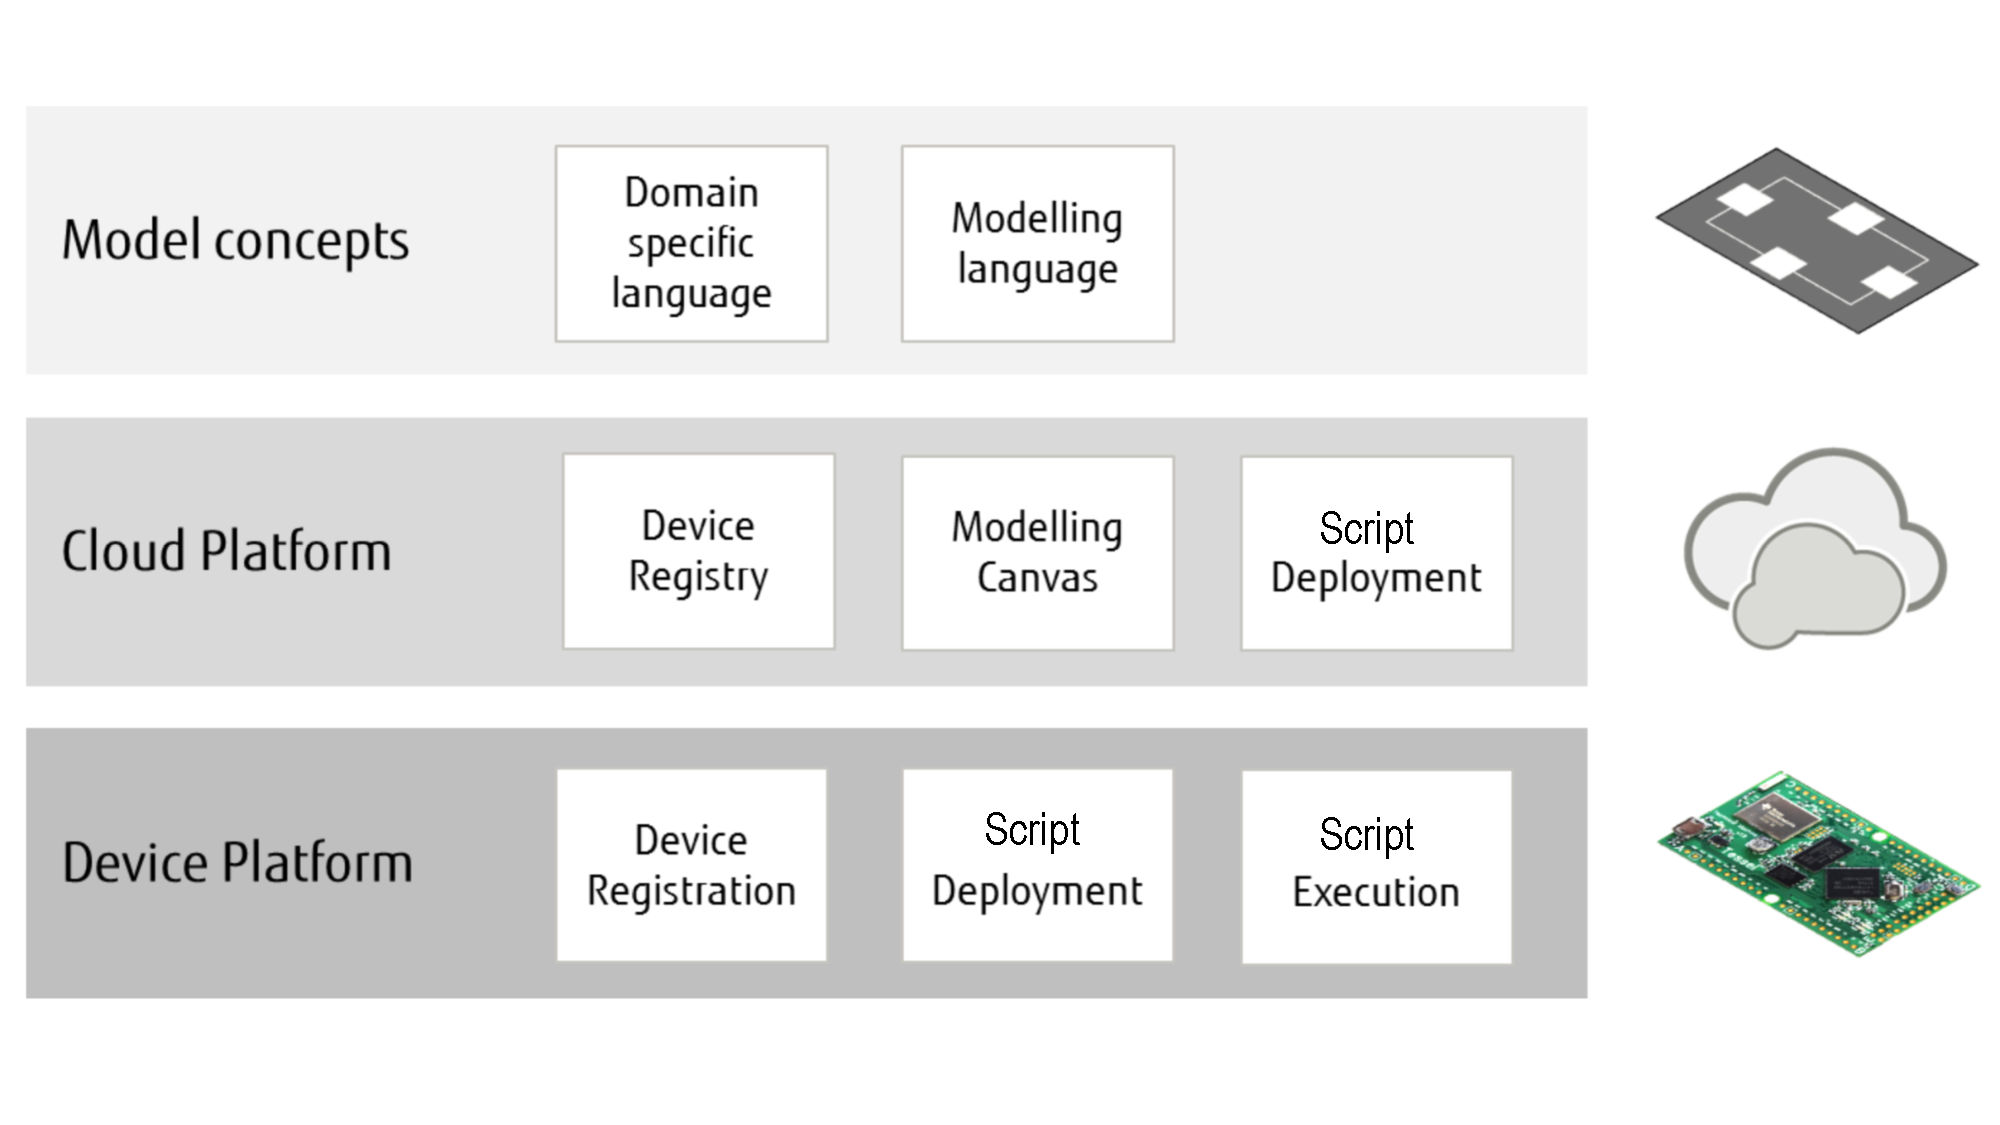
\includegraphics[width=0.8\linewidth]{Figures/sample-figure}
% 	\caption[]{Sample figure.}
% 	\label{fig:sample-figure}
% \end{figure}
